\usetikzlibrary{calc}

\newcommand{\cartpole}[3]{
	\fill[#1] (#2-0.5,0) rectangle (#2 + 0.5, 0.5); % Base
    \draw[line width=1.5,#1] (#2,0.5) -- +(#3:2); % Pole
}

\newcommand{\cartpoleCWF}[5]{
	\cartpole{#1}{#2}{#3};
    \draw[color=white,->] (#2-0.2,0.25)  -- (#2+0.2,0.25);
	\draw[<-] ($(#2,0.5)  +(#3-10:2) $) arc (#3-20:#3+20:1);
	\node[above,rotate=#3-90] at ($(#2,0.5)  +(#3:2) $) {#5}; 
	\node[below] at (#2,0.0) {#4};
}
\newcommand{\cartpoleCCWF}[5]{
	\cartpole{#1}{#2}{#3};
    \draw[color=white,->] (#2-0.2,0.25)  -- (#2+0.2,0.25);
	\draw[->] ($(#2,0.5)  +(#3-10:2) $) arc (#3-20:#3+20:1); 
	\node[above,rotate=#3-90] at ($(#2,0.5)  +(#3:2) $) {#5}; 
	\node[below] at (#2,0.0) {#4};
}
\newcommand{\cartpoleCWB}[5]{
	\cartpole{#1}{#2}{#3};
    \draw[color=white,<-] (#2-0.2,0.25)  -- (#2+0.2,0.25);
	\draw[<-] ($(#2,0.5)  +(#3-10:2) $) arc (#3-20:#3+20:1);
	\node[above,rotate=#3-90] at ($(#2,0.5)  +(#3:2) $) {#5}; 
	\node[below] at (#2,0.0) {#4};
}
\newcommand{\cartpoleCCWB}[5]{
	\cartpole{#1}{#2}{#3};
    \draw[color=white,<-] (#2-0.2,0.25)  -- (#2+0.2,0.25);
	\draw[->] ($(#2,0.5)  +(#3-10:2) $) arc (#3-20:#3+20:1); 
	\node[above,rotate=#3-90] at ($(#2,0.5)  +(#3:2) $) {#5}; 
	\node[below] at (#2,0.0) {#4};
}
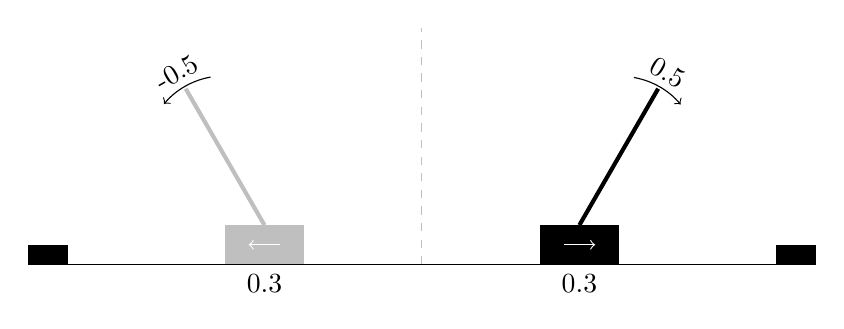
\begin{tikzpicture}

\draw[dashed,color=lightgray] (0,0) -- (0,3);
\cartpoleCWF{}{2}{60}{0.3}{0.5};
\cartpoleCCWB{color=lightgray}{-2}{120}{0.3}{-0.5};


\draw (-5,0) -- (5,0); % Ground
\fill (-5,0) rectangle (-4.5,0.25);
\fill (5,0) rectangle (4.5,0.25);

\end{tikzpicture}